\chapter{Solução Proposta}

\section{Apresentação}

A solução materializa-se numa plataforma web para anotação de dados de chat, com foco inicial no processo de disentanglement. O desenvolvimento baseou-se num protótipo funcional \cite{prototype} que permitiu validar conceitos base e estabelecer fundações para evolução futura.

\paragraph{Protótipo Inicial}
O protótipo, desenvolvido entre outubro e novembro de 2024, implementou funcionalidades essenciais:

\begin{itemize}
    \item Interface base de visualização de chat
    \item Sistema de gestão de tags para anotação
    \item Processamento de ficheiros CSV com formato específico
    \item Gestão básica de workspace para ficheiros
\end{itemize}

\paragraph{Requisitos de Dados}
O sistema processa ficheiros CSV com estrutura específica, incluindo:

\begin{itemize}
    \item user\_id: identificador do utilizador
    \item turn\_id: identificador único da mensagem
    \item turn\_text: conteúdo da mensagem
    \item reply\_to\_turn: referência explícita a outra mensagem
    %\item thread: identificação da thread (preenchido pelo anotador)
\end{itemize}

\paragraph{Insights do Protótipo}
O desenvolvimento exploratório inicial proporcionou descobertas importantes:

\begin{itemize}
    \item Validação da interface de anotação para disentanglement
    \item Confirmação da viabilidade do processamento de ficheiros CSV
    \item Identificação de pontos de optimização no fluxo de trabalho
    \item Feedback directo dos utilizadores sobre funcionalidades essenciais
\end{itemize}

\section{Arquitectura}

A arquitectura da solução, representada na Figura~\ref{fig:diagrama-arquitectura}, incorpora elementos de diferentes abordagens analisadas no benchmarking. Esta decisão reflecte-se em dois princípios base:

\paragraph{Operacionalização}
O primeiro foca-se na operacionalização através de:

\begin{itemize}
    \item Deployment via containers para simplicidade operacional
    \item Configuração reduzida para facilitar manutenção
    \item Monitorização integrada de componentes
    \item Backup e recuperação de dados simplificados
\end{itemize}

\paragraph{Modularidade}
O segundo centra-se na modularidade através de:

\begin{itemize}
    \item Interfaces bem definidas entre componentes
    \item Separação clara de responsabilidades
    \item Sistema de plugins para extensões
    \item Gestão independente de dados por módulo
\end{itemize}

\paragraph{Evolução Planeada}
A arquitectura suporta evolução em várias dimensões:

\begin{itemize}
    \item Adição de novos módulos de anotação
    \item Integração com ferramentas de análise
    \item Expansão das capacidades de processamento
    \item Adaptação a diferentes tipos de dados
\end{itemize}

\section{Tecnologias e Ferramentas Utilizadas}

A implementação assenta em tecnologias web estabelecidas, escolhidas conforme estado da arte e conforme os requisitos do projeto. O frontend utiliza React para a interface de anotação, enquanto o backend em Python gere o processamento de dados, permitindo integração eficiente com ferramentas de análise e processamento.

\paragraph{Frontend}
A escolha do React como framework principal mantém-se desde o protótipo inicial, fundamentada por:

\begin{itemize}
    \item Gestão eficiente de estado através de Hooks
    \item Componentes reutilizáveis para consistência da interface
    \item Rendering optimizado para operações frequentes
    \item Extensa documentação e comunidade activa
\end{itemize}

\paragraph{Backend}
O desenvolvimento em Python permite:

\begin{itemize}
    \item Integração com bibliotecas de processamento de dados
    \item Implementação eficiente de métricas e análises
    \item Alinhamento com o ecossistema do departamento
    \item Extensibilidade para funcionalidades futuras
\end{itemize}

\section{Ambientes de Teste e de Produção}

O desenvolvimento segue uma abordagem iterativa com dois ambientes distintos:

\paragraph{Ambiente de Desenvolvimento}
Suporta o desenvolvimento activo e testes:

\begin{itemize}
    \item Configuração simplificada para desenvolvimento local
    \item Dados de teste para validação de funcionalidades
    \item Ferramentas de debugging e monitorização
    \item Automatização de testes unitários e de integração
\end{itemize}

\paragraph{Ambiente de Produção}
Garante estabilidade e performance:

\begin{itemize}
    \item Configuração optimizada para performance
    \item Backup automático de dados
    \item Monitorização de métricas operacionais
    \item Gestão de logs e diagnóstico
\end{itemize}

\section{Abrangência}

A solução abrange inicialmente o processo de disentanglement de conversas em chatrooms, estabelecendo bases para expansão futura. A arquitectura modular permite adicionar novos tipos de anotação sem alterações estruturais significativas.

\paragraph{Módulo de Disentanglement}
O primeiro módulo implementado foca-se em:

\begin{itemize}
    \item Interface especializada para visualização de chatrooms
    \item Ferramentas para identificação e separação de conversas
    \item Sistema de validação de anotações
    \item Métricas de progresso e qualidade
\end{itemize}

\paragraph{Extensibilidade}
A arquitectura suporta expansão através de:

\begin{itemize}
    \item Interfaces bem definidas para novos módulos
    \item Gestão independente de dados por módulo
    \item Documentação para desenvolvimento de extensões
\end{itemize}

\section{Componentes}

\subsection{Frontend}

O frontend da aplicação assenta em React 18, escolha fundamentada pela experiência bem-sucedida do protótipo inicial e pelas capacidades da framework para desenvolvimento de interfaces complexas. A implementação aproveita características modernas do React, como Hooks e componentes funcionais, permitindo uma gestão de estado eficiente e código mais manutenível.

A arquitectura do frontend organiza-se em componentes modulares, cada um com responsabilidades bem definidas:

\paragraph{Sistema de Componentes}
O desenvolvimento segue uma abordagem baseada em componentes reutilizáveis, organizados em três níveis:

\begin{itemize}
    \item \textbf{Componentes Base}: Elementos UI fundamentais como botões, inputs e cards, implementados com styled-components para consistência visual
    \item \textbf{Componentes Compostos}: Agregações de componentes base que implementam funcionalidades específicas, como o visualizador de mensagens ou o sistema de tagging
    \item \textbf{Páginas}: Composições completas que integram múltiplos componentes para criar interfaces funcionais
\end{itemize}

\paragraph{Gestão de Estado}
A gestão de estado utiliza uma combinação de React Hooks nativos e contextos, evitando a complexidade adicional de soluções como Redux. Esta decisão baseou-se na experiência do protótipo, onde se verificou que:

\begin{itemize}
    \item O estado local com useState é suficiente para a maioria dos componentes
    \item useContext permite compartilhar estado eficientemente entre componentes relacionados
    \item useReducer oferece gestão de estado mais complexa quando necessário
\end{itemize}

\paragraph{Interface de Anotação}
O componente central da aplicação - a interface de anotação - foi redesenhado com base no feedback do protótipo. Implementa:

\begin{itemize}
    \item Visualização em split-view das mensagens e threads identificadas
    \item Sistema de drag-and-drop para classificação de mensagens
    \item Preview em tempo real das alterações
    \item Atalhos de teclado para operações frequentes
\end{itemize}

\subsection{Backend}

O backend da aplicação será desenvolvido em Python, escolha fundamentada pela necessidade de integração com ferramentas de processamento de dados e análise. A implementação utilizará uma web framework Python moderna (Flask ou FastAPI), permitindo o desenvolvimento de uma API REST robusta e eficiente.

\paragraph{Arquitectura do Backend}
O backend segue uma arquitectura em camadas:

\begin{itemize}
    \item \textbf{API Layer}: Implementação de endpoints REST utilizando uma web framework Python (Flask ou FastAPI)
    \item \textbf{Service Layer}: Lógica de negócio e processamento de dados
    \item \textbf{Data Layer}: Gestão de persistência e acesso a dados
\end{itemize}

\paragraph{Processamento de Dados}
O sistema implementa um pipeline de processamento específico para chatrooms:

\begin{itemize}
    \item Parsing e validação de ficheiros CSV
    \item Estruturação de conversas em formato adequado para anotação
    \item Cálculo de métricas e estatísticas
    \item Cache de resultados frequentes
\end{itemize}

\paragraph{Sistema de Persistência}
A persistência de dados será implementada utilizando uma base de dados SQL leve como SQLite, através de um ORM para Python. Esta abordagem permite:

\begin{itemize}
    \item Gestão eficiente de dados estruturados
    \item Queries optimizadas para diferentes volumes de dados
    \item Backup e versionamento de dados
\end{itemize}

\subsection{Fluxo de Dados}

O fluxo de dados na plataforma foi desenhado para reflectir as necessidades práticas do processo de anotação:

\paragraph{Importação}
Os administradores podem carregar ficheiros CSV contendo conversas de chatrooms. O processo é deliberadamente simplificado, permitindo:

\begin{itemize}
    \item Upload directo de ficheiros
    \item Validação automática do formato
    \item Feedback imediato sobre a qualidade dos dados
\end{itemize}

\paragraph{Processamento}
O backend processa os ficheiros, preparando-os para anotação:

\begin{itemize}
    \item Validação estrutural dos dados
    \item Organização das mensagens em sequência temporal
    \item Preparação para disentanglement
\end{itemize}

\paragraph{Distribuição}
As conversas são disponibilizadas através da interface web:

\begin{itemize}
    \item Atribuição automática aos anotadores
    \item Tracking de progresso
    \item Sistema de validação em tempo real
\end{itemize}

\section{Interfaces}

A comunicação entre componentes realiza-se através de uma API REST, permitindo independência entre frontend e backend. Esta abordagem facilita:

\begin{itemize}
    \item Desenvolvimento paralelo de componentes
    \item Manutenção e evolução independente
    \item Integração com ferramentas externas
    \item Testes isolados de funcionalidades
\end{itemize}

O sistema de dados organiza-se por módulos, onde cada tipo de anotação mantém seu próprio modelo de dados. Para o disentanglement, isto inclui:

\begin{itemize}
    \item Estrutura de dados optimizada para chatrooms
    \item Sistema de versionamento de anotações
    \item Métricas específicas para avaliação
    \item Export em formatos standard
\end{itemize}

O diagrama apresentado na Figura~\ref{fig:diagrama-arquitectura} detalha os principais componentes da solução, incluindo o frontend em React, backend em Python, sistema de persistência de dados e as interfaces de comunicação entre os diferentes módulos. A arquitectura modular permite a extensão futura com novos tipos de anotação além do módulo inicial de disentanglement.

\begin{landscape}
    \begin{figure}[p]
        \centering
        \makebox[\textwidth][c]{%
            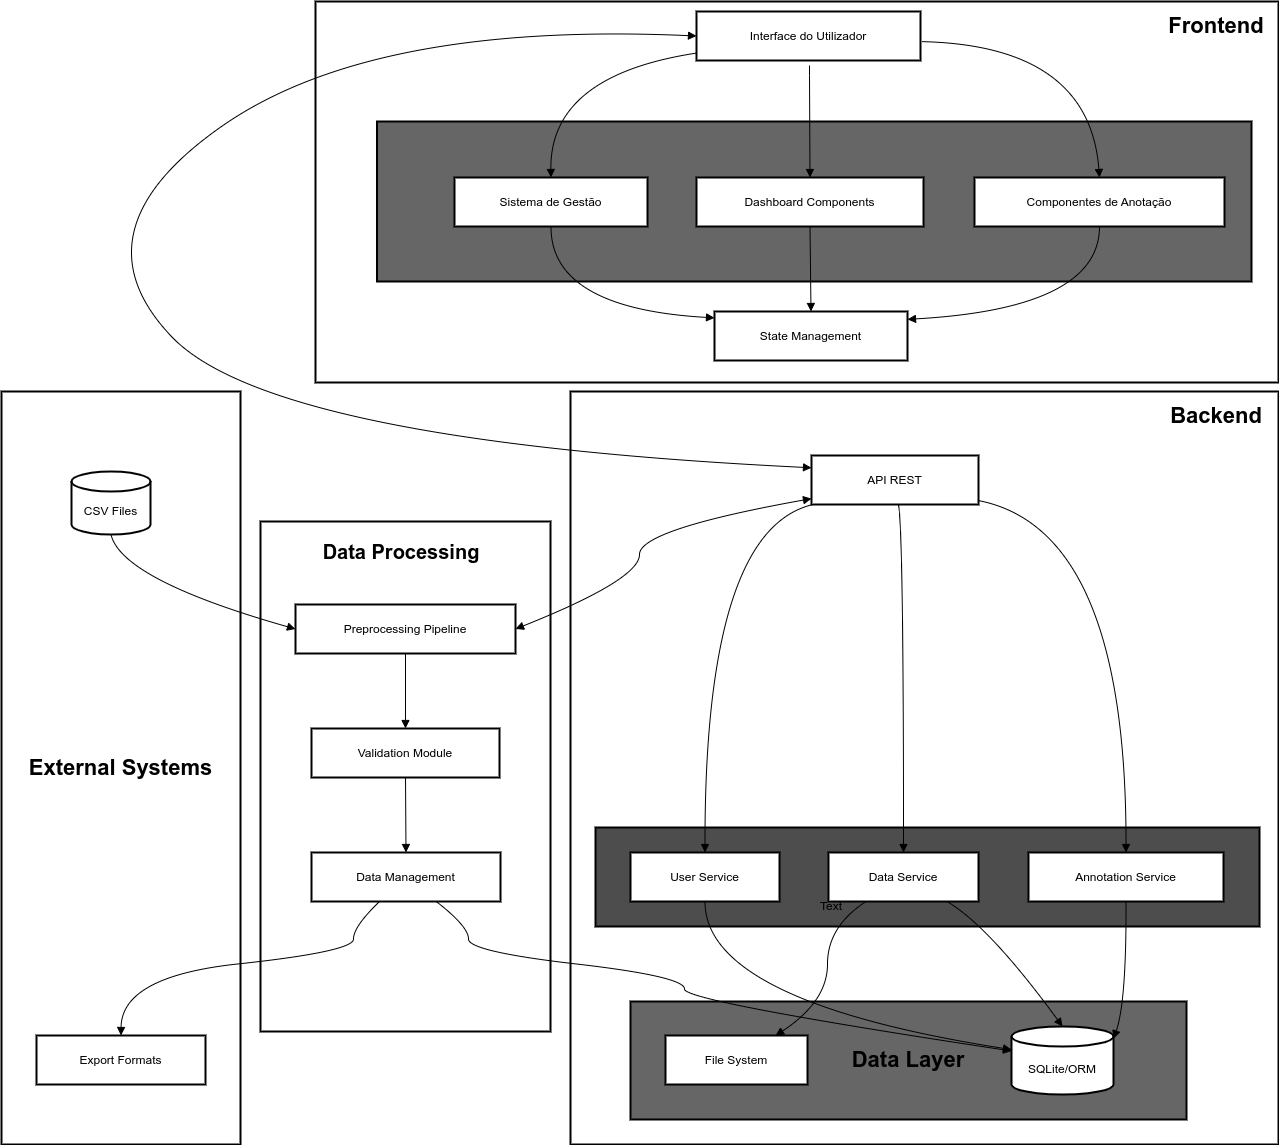
\includegraphics[width=0.60\paperheight, angle=0, keepaspectratio]{images/diagramaArquitetura.drawio.png}
        }
        \caption{Diagrama de Arquitectura do Sistema.}
        \label{fig:diagrama-arquitectura}
    \end{figure}
\end{landscape}